\documentclass[12pt]{article}
\renewcommand{\baselinestretch}{1.2} 	% line Spacing
\usepackage{geometry}
\geometry{margin=1.25in}

\title{\bf \Huge{BnfCalculator} \\ \large{An Exercise in Parsing}}
\author{John~Till}
\date{}

\usepackage[]{hyperref}
\hypersetup{
    pdftitle={Title},
    pdfauthor={John Till},
    pdfsubject={Parsing},
    pdfkeywords={Knoxville Papers, Parsing, Rewriting, Big-num},
    bookmarksnumbered=true,     
    bookmarksopen=true,         
    bookmarksopenlevel=1,       
    colorlinks=true,            
    pdfstartview=Fit,           
    pdfpagemode=UseOutlines,    % this is the option you were lookin for
    pdfpagelayout=TwoPageRight
}

\usepackage[nounderscore]{syntax}
\makeatletter
\def\gr@implitem#1<#2> #3 {%
	\sbox\z@{\hskip\labelsep\grammarlabel{#2}{#3}}%
	\strut\@@par%
	\vskip-\parskip%
	\vskip-\baselineskip%
	\hrule\@height\z@\@depth\z@\relax%
	\item[\unhbox\z@]%
	\catcode`\<\active%
}
\makeatother

\usepackage{float}                      % figure floats
\usepackage[numbers]{natbib}                     % this package allows you to link your references
\usepackage{graphicx}					% graphics package
\usepackage{fancyhdr}                   % fancy headers and footers
\usepackage[inactive]{srcltx}		 	% necessary to use forward and inverse searching in DVI
\usepackage{relsize}                    % font sizing hierarchy
\usepackage{booktabs}                   % professional looking tables
\usepackage[config, labelfont={bf}]{caption,subfig} % nice sub figures
\usepackage{mathrsfs}                   % additional math scripts
\usepackage{eufrak}
\usepackage[titletoc]{appendix}			% format appendix correctly
\usepackage{pdflscape}					% to produce landscape pages if necessary

\usepackage{amsfonts}
\usepackage{mathtools}
\usepackage{empheq}
\usepackage{pdfsync}
\usepackage{flushend}
\usepackage{verbatim}
\usepackage{algorithm}
\usepackage{algorithmic}
\usepackage{mathrsfs}
\usepackage{cancel}
\usepackage{enumitem}
\usepackage{rotating} %sidewaysfigure

\usepackage{listings,textcomp,xcolor}
\lstdefinestyle{defaultStyle}
{
  basicstyle=\footnotesize,
  tabsize=2,
  captionpos=b,
  frame=lines,
  breaklines=true,
  keepspaces=true
}
% define C++ style
\lstdefinestyle{cppStyle}
{
  style=defaultStyle,
  % language related
  language=C++,
  keywordstyle=\color{violet},
  commentstyle=\color{green},
  stringstyle=\color{gray},
  showstringspaces=false,
  %otherkeywords={\#include}, % do not uncomment!
  % numbering
  numbers=left,
  numberstyle=\tiny
}
\lstset{emph={%  
    real_type%
    },emphstyle={\color{violet}}%
}%

\lstdefinestyle{MATLAB}
{
		language=MATLAB,%
		basicstyle=\fontsize{8}{10}\ttfamily,
    %basicstyle=\color{red},
    breaklines=true,%
    %morekeywords={matlab2tikz},
    keywordstyle=\color{blue},%
		%keywordstyle=[1]\color{black},
    morekeywords=[2]{1}, keywordstyle=[2]{\color{black}},
    identifierstyle=\color{black},%
    stringstyle=\color{violet},
    commentstyle=\color{green},%
    showstringspaces=false,%without this there will be a symbol in the places where there is a space
    numbers=left,%
    numberstyle={\tiny \color{black}},% size of the numbers
    numbersep=9pt, % this defines how far the numbers are from the text
    emph=[1]{for,end,break},emphstyle=[1]\color{red}, %some words to emphasise
    %emph=[2]{word1,word2}, emphstyle=[2]{style},
		lineskip={-1.7pt}
}

\newcommand{\sgn}{\operatorname{sgn}}
\newcommand{\norm}[1]{\left\lVert#1\right\rVert}
%\newcommand{\bf}[1]{\boldsymbol{#1}}

\newcommand{\nomunit}[1]{%
\renewcommand{\nomentryend}{\hspace*{\fill}#1}}

%Grammar commands to use with align environment
\definecolor{terminalcolor}{RGB}{0, 185, 202}
\definecolor{nonterminalcolor}{RGB}{0, 99, 169}
\definecolor{directcolor}{RGB}{115, 65, 10}
\newcommand{\customgrammar}[1]{
\begin{align*}
#1
\end{align*}
}
\newcommand{\finishrule}{}
\newcommand{\orinline}{\;\;|\;\;}
\newcommand{\orbreak}{&\;\;\;|\;\;}
\newcommand{\terminal}[1]{\text{\textcolor{terminalcolor}{#1}}}
\newcommand{\nonterminal}[1]{\text{\textcolor{nonterminalcolor}{#1}}}
\newcommand{\direct}[1]{\text{`\textcolor{directcolor}{#1}'}}

%%%%%%%%%%%%%%%%%%%%%%%%%%%%%%%%%%%%%%%%%%%%%%%%%%%%%%%%%%%%%%%%%%%%%%%%%%%%%%%%%%%%%%%%%%%%%%%%%%%%%
\begin{document}
	\pagenumbering{alph} % this is needed to clear certain issues with the hyperref package
	\pagenumbering{roman}
	\setcounter{page}{2}

	\maketitle

	\pagenumbering{arabic}
	\setcounter{page}{1}

\section{Numeric Expressions}

One of the quickest tasks to test our parsing abilities is to build a calculator, which requires us to parse and evaluate mathematical expressions. There are three components we will use-- a scanner, parser, and abstract syntax tree (AST). The types of expressions which are parsed are summarized in the following BNF grammar:

\customgrammar{
\nonterminal{Expression} &\Rightarrow \nonterminal{Below} \finishrule \\
\nonterminal{Addition} &\Rightarrow \nonterminal{Below} \; ((\direct{+} \orinline \direct{-}) \; \nonterminal{Below})* \finishrule \\
\nonterminal{Multiplication} &\Rightarrow \nonterminal{Below} \; ((\direct{*} \orinline \direct{/} \orinline \direct{$\backslash$} \orinline \direct{$\%$}) \; \nonterminal{Below})* \finishrule \\
\nonterminal{LeftUnary} &\Rightarrow \direct{-}* \; \nonterminal{Below} \finishrule \\
\nonterminal{RightUnary} &\Rightarrow \nonterminal{Below} \; \direct{!}* \finishrule \\
\nonterminal{Exponent} &\Rightarrow \nonterminal{Below} \; (\direct{\^{}} \; \nonterminal{LeftUnary})? \finishrule \\
\nonterminal{Primitive} &\Rightarrow \nonterminal{Grouping} \orinline \nonterminal{AbsoluteValue} \orinline \terminal{NumberLiteral} \orinline \nonterminal{Call} \finishrule \\
\nonterminal{Grouping} &\Rightarrow \direct{(} \; \nonterminal{Expression} \direct{)} \finishrule \\
\nonterminal{AbsoluteValue} &\Rightarrow \direct{$|$} \; \nonterminal{Expression} \; \direct{$|$} \finishrule \\
\nonterminal{Call} &\Rightarrow \terminal{Identifier} \; \nonterminal{CallArgs}? \finishrule \\
\nonterminal{CallArgs} &\Rightarrow \direct{(} \; (\nonterminal{Expression} \; (\direct{,} \; \nonterminal{Expression})*)? \; \direct{)} \finishrule \\
&\\
\terminal{NumberLiteral} &\Rightarrow (\direct{0}-\direct{9})+ \; (\direct{.} \; (\direct{0}-\direct{9})+)? \finishrule \\
\terminal{Identifier} &\Rightarrow (\direct{a}-\direct{z} \orinline \direct{A}-\direct{Z}) \; (\direct{a}-\direct{z} \orinline \direct{A}-\direct{Z} \orinline \direct{0}-\direct{9})* \finishrule
}

Fortunately the only rules with repeated symbols are numbers, started with a digit, or variables, started with a letter. Any other symbol encountered can be directly mapped to a token type by the scanner. There are just a few keywords-- ``pi'', ``cos'', ``sin'', ``tan'', ``e'', ``ln'', and ``log''. Tokens for each keyword are actually built into the grammar, although that detail is ignored in the prior BNF grammar. The parser is a simple recursive descent parser.

The AST uses an OOP design with a pure virtual ``eval'' function. While this isn't a great design for parsing numeric expressions, it will be a useful abstraction later as the number of pure virtual functions grows.

\begin{figure}[h]
	\centering
		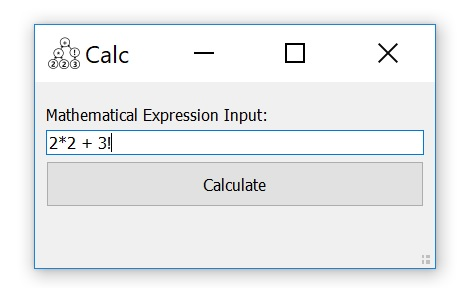
\includegraphics[width=0.50\textwidth]{Fig/Screenshot.jpg}
	\label{fig:screenshot}
\end{figure}

\section{Symbolic Expressions}

There are a couple more drills to practice by tacking on a symbolic mode to the calculator. First, big-num arithmetic is implemented in ``numbers.h''. A big unsigned integer is represented by a STL vector of uint8\_t entries. Each element represents a single digit of the big integer, and the order is so that the first element corresponds to the rightmost digit, i.e. forward traversal of the vector visits the big int from right to left. It is a fairly naive implementation, but the implementation details are encapsulated well, and the solution is straightforward.

The second skill exercised is rewriting. Transformations are implemented directly in the AST as a pure virtual method to be defined by each specific node. This is not ideal to allow the AST to scale or to implement complicated transformation rules relying on many nodes (e.g. $\sin(x)^2 + \cos(x)^2 \Rightarrow 1$), but it allows us to play around with a few transformations without painstakingly defining a generalization of rewriting rules.

\begin{figure}[h]
	\centering
		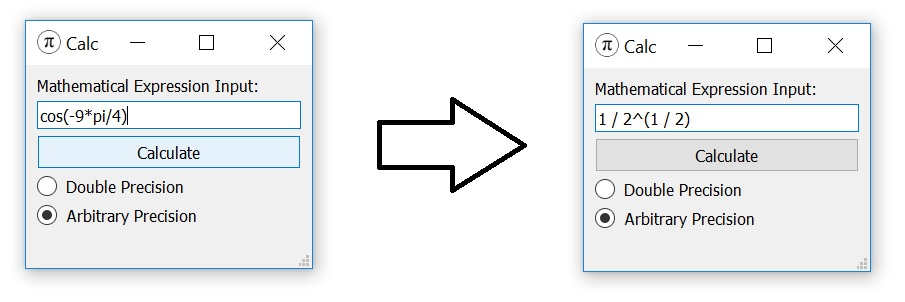
\includegraphics[width=1.00\textwidth]{Fig/Symbolic.jpg}
	\label{fig:symbolic}
\end{figure}

\section{Conclusions}

This is a good exercise to work on parsing, rewriting, and big-num arithmetic. The calculator app is free from any statement grammar or symbol table, and the symbolic mode is kept simple by allowing parent nodes to transform based on child types.

\end{document}
